% Asset ID: AS2StatisticalSamplingTIKZ-002
% Unit: AS2 Applied Mathematics
% Topic: AS2-SAMP Statistical sampling
% Purpose: Census vs sample comparison
% Source: Supplied Data Collection PDF page 7 and transcript Data Collection 1
% Linked LO IDs: AS2-SAMP-LO001, AS2-SAMP-LO002, AS2-SAMP-LO004

\documentclass[tikz,border=8pt]{standalone}
\usetikzlibrary{positioning,fit}
\begin{document}
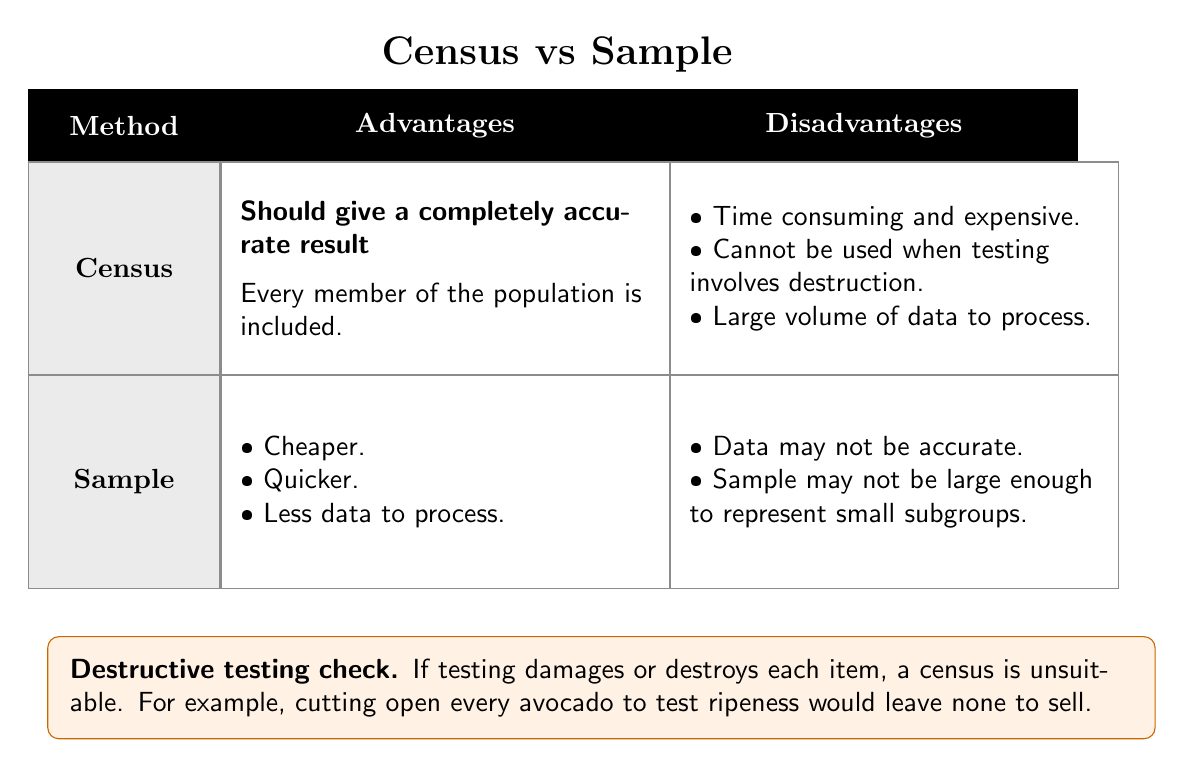
\begin{tikzpicture}[
  font=\sffamily,
  header/.style={draw=black,fill=black,text=white,font=\bfseries,align=center,minimum height=0.9cm},
  cell/.style={draw=black!45,fill=white,align=left,text width=5.2cm,minimum height=2.7cm,inner sep=7pt},
  method/.style={draw=black!45,fill=black!8,align=center,font=\bfseries,text width=2.2cm,minimum height=2.7cm},
  warning/.style={draw=orange!80!black,fill=orange!10,rounded corners=4pt,text width=13.5cm,align=left,inner sep=8pt}
]
\node[font=\bfseries\Large] at (6.6,5.25) {Census vs Sample};
\node[header,text width=2.2cm] (h1) at (1.1,4.35) {Method};
\node[header,text width=5.2cm,right=0cm of h1] (h2) {Advantages};
\node[header,text width=5.2cm,right=0cm of h2] (h3) {Disadvantages};
\node[method,below=0cm of h1] (m1) {Census};
\node[cell,right=0cm of m1] (a1){\textbf{Should give a completely accurate result}\\[2mm]Every member of the population is included.};
\node[cell,right=0cm of a1] (d1){\textbullet\ Time consuming and expensive.\\\textbullet\ Cannot be used when testing involves destruction.\\\textbullet\ Large volume of data to process.};
\node[method,below=0cm of m1] (m2) {Sample};
\node[cell,right=0cm of m2] (a2){\textbullet\ Cheaper.\\\textbullet\ Quicker.\\\textbullet\ Less data to process.};
\node[cell,right=0cm of a2] (d2){\textbullet\ Data may not be accurate.\\\textbullet\ Sample may not be large enough to represent small subgroups.};
\node[warning,below=0.6cm of m2.south east,anchor=north west,xshift=-2.2cm] (w){\textbf{Destructive testing check.} If testing damages or destroys each item, a census is unsuitable. For example, cutting open every avocado to test ripeness would leave none to sell.};
\end{tikzpicture}
\end{document}
